\documentclass[12 pt]{article}

% Fonts/Symbols/Colors
\usepackage{fullpage}
\usepackage{amsthm}
\usepackage{amsmath}
\usepackage{xcolor}
\usepackage{amssymb}
\usepackage{verbatim}
\usepackage{graphicx}
\usepackage[utf8x]{inputenc}
\usepackage{helvet}
\renewcommand{\familydefault}{\sfdefault}

% Question counter
\newcounter{qnum}

% Question Formatting
\newcommand{\new}[1]{\bigskip \noindent \color{blue} \textbf{#1}\medskip}
\newcommand{\response}[1]{\color{black} #1 \medskip}
\newcommand{\q}[1]{\response{\emph{#1}}}
\newcommand{\Q}[1]{\stepcounter{qnum}\new{Goal {\arabic{qnum}}:} \q{#1}}

% INSERT WEEK NUMBER HERE
\newcommand{\setnum}{1}

\begin{document}

% Title Section
\begin{center}
    \Large \color{blue} CS134: Robotics Systems\color{black}
    \begin{center}\normalsize Team GLaDOS Weekly Report \setnum{}\end{center}
    \noindent{\color{black} \rule{\linewidth}{0.5mm} }
\end{center}

% Body
\textbf{Progress}:
    \begin{enumerate}
        \item The robot hardware setup was improved over last week's setup:
            \begin{itemize}
                \item The robot power and NUC were placed underneath the table to 
                give the robot a fully unobstructed workspace.
                \item The robot cables were organized and secured around the joints, and 
                full range of motions verified to be unobstructed by the cables.
            \end{itemize}
        \item The robot dimensions were measured and placed into the URDF file which 
        was verified in Rviz.
        \item Using the KinematicChain code from 133A, the robot kinematics were
        coded using a weighted psuedoinverse to provide robustness to singularities.
        \item The robot was able to move to both joint positions and cartesian positions
        in the workspace.
        \item A demo was created in which the robot takes in positions given at any time
        from ROS commands and moves to that goal and then back to the waiting position. The 
        software builds up a queue of goals and moves to them in order, or waits at the ready 
        position if there are no goals in the queue.
        \item A gravity compensation controller was implemented to allow the robot to
        resist the strength of gravity. We found the value of our constants to be $A=-1.8$ and $B=0.4$
        \item We created plots to verify the tracking of the actual joint positions, velocities, and efforts to 
        those which were commanded.
    \end{enumerate}
    \begin{center}
        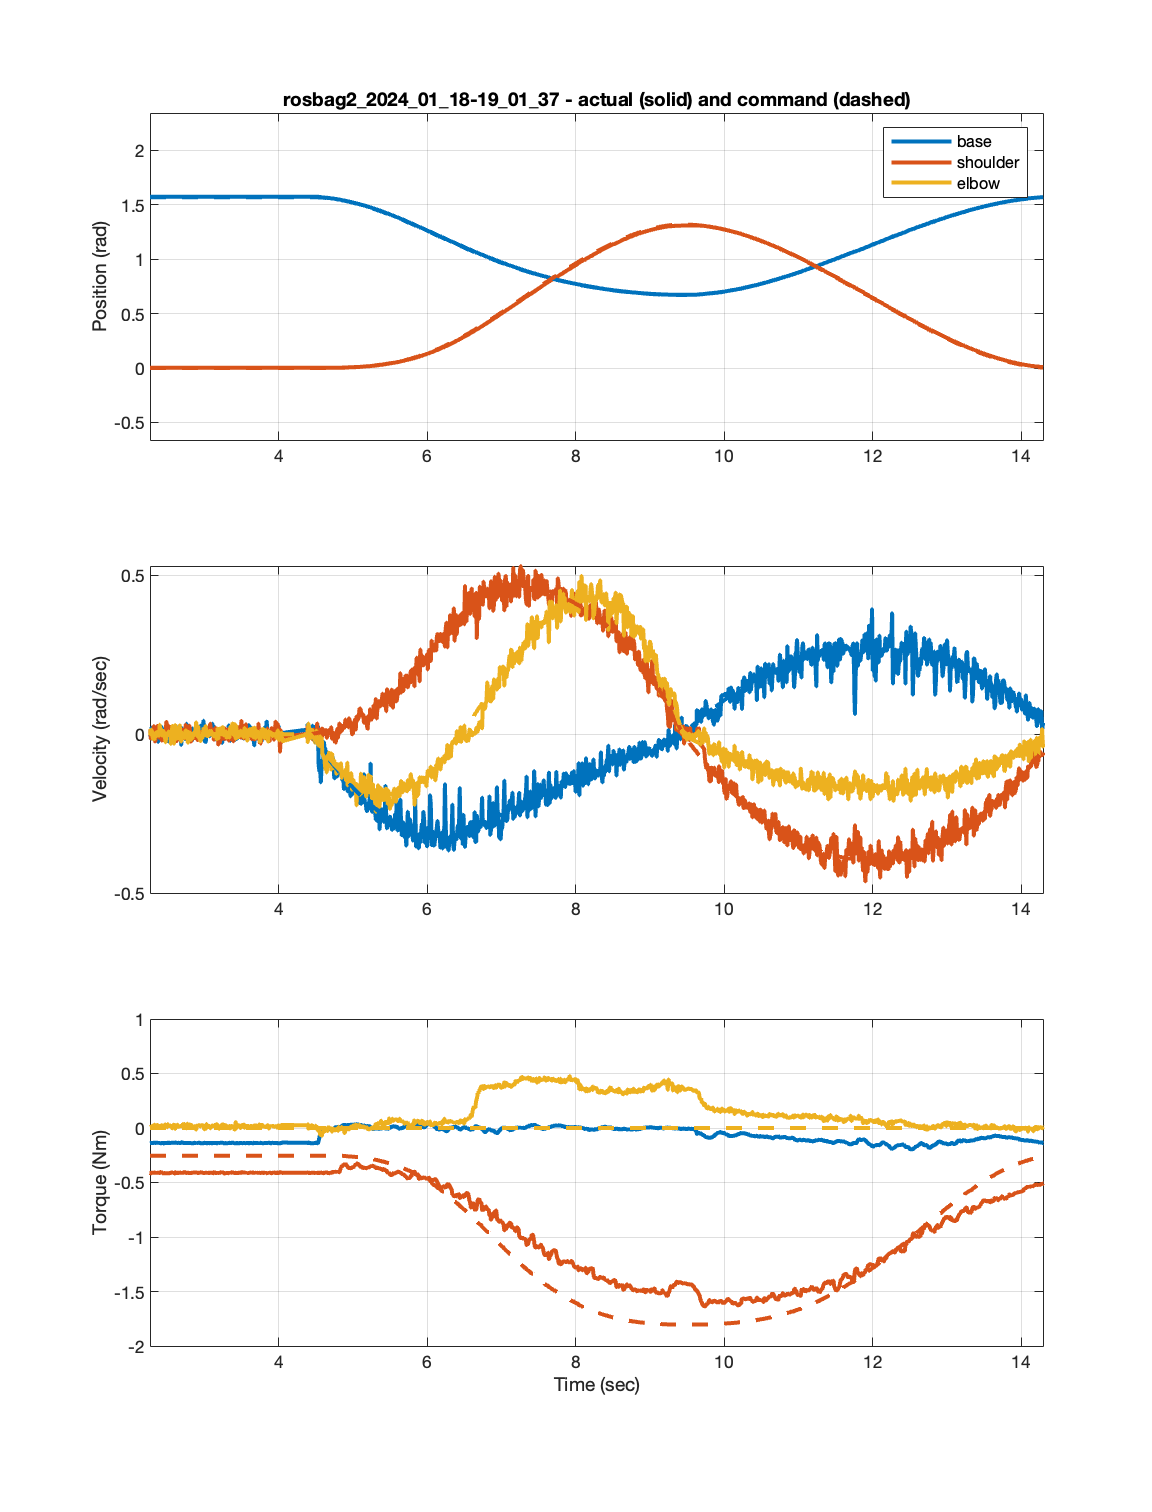
\includegraphics[scale=0.7]{actualvscommand.png} \\
        \emph{Joint tracking with a collision at t=6.4}
    \end{center}

\textbf{To-Do}:
    \begin{itemize}
        \item Improve the callibration of the robot to match the task space to the joint space. 
        Currently the joints track well to their commanded positions but the corresponding tip 
        position is off from expected by up to half a centimeter.
        \item Implement contact detection
    \end{itemize}

\textbf{Issues}:
    \begin{itemize}
        \item We improved a lot of issues with measurements between the URDF and
        the actual robot which greatly improved the callibration of the robot and 
        its task space position, but now we are unsure where the remining error
        stems from. 
    \end{itemize}

\end{document}